\section{Ejemplos.}
\subsection{Visualizando algunas iteraciones}
Como primer ejemplo para visualizar el algoritmo se puede utilizar el polinomio deducido en
(\refeq{muller_order_eq}) y encontrar todas sus raíces haciendo uso del algoritmo. Primero se presenta
una gráfica del polinomio como función compleja, representando en los ejes $x,y$ de la gráfica el plano
complejo y en el eje $z$ de la gráfica el módulo de cada valor de la función, tal representación resulta útil para visualizar
dónde se encuentran las raíces en el plano complejo. Las tres raíces del polinomio con seis decimales 
correctos son: 
\begin{align*}
    \left(+1.839286+0.000000i\right)\\(-0.419643-0.606290i)\\(-0.419643+0.606290i)
\end{align*}
Una gráfica de dicho polinomio puede verse en la figura \refeq{zero_poly} (con $z$ siendo un número complejo).
Se consideran algunas iteraciones del método de Muller con su respectiva forma y sus raíces de modo que se pueda visualizar
su comportamiento y sucesiva aproximación a una de las raíces. Eligiendo los puntos más cercanos a cada raíz
es posible utilizar el método para encontrarlas todas.


\begin{figure}
    \centering
    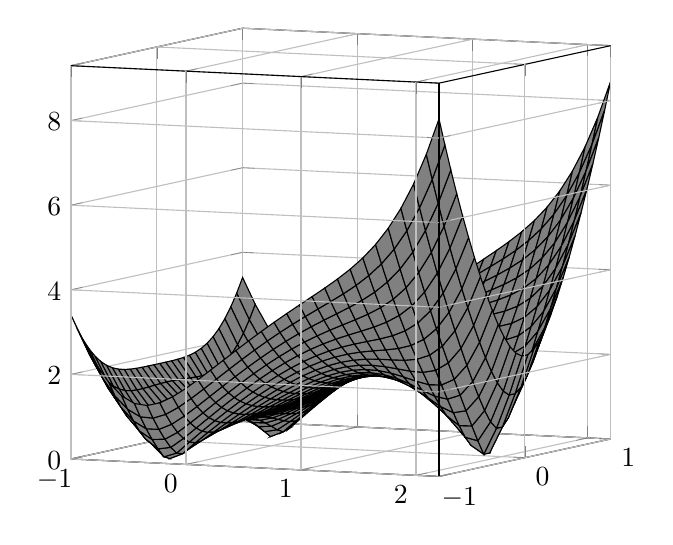
\begin{tikzpicture}
        \begin{axis}[view={25}{6},zmin=0,grid,
            3d box = complete*]
        \addplot3 [
            domain=-1:2.2,
            domain y = -1:1,
            samples = 30,
            samples y = 30,
            surf,
            fill=black!50,
            faceted color=black] {((3*x^2*y-2*x*y-y^3-y)^2+(x^3-x^2-3*x*y^2-x+y^2-1)^2)^(1/2)-0.2};
        \end{axis}
    \end{tikzpicture}
    \caption{Polinomio $z^3-z^2-z-1$}
    \label{zero_poly}
\end{figure} 
\begin{figure}
    \centering
    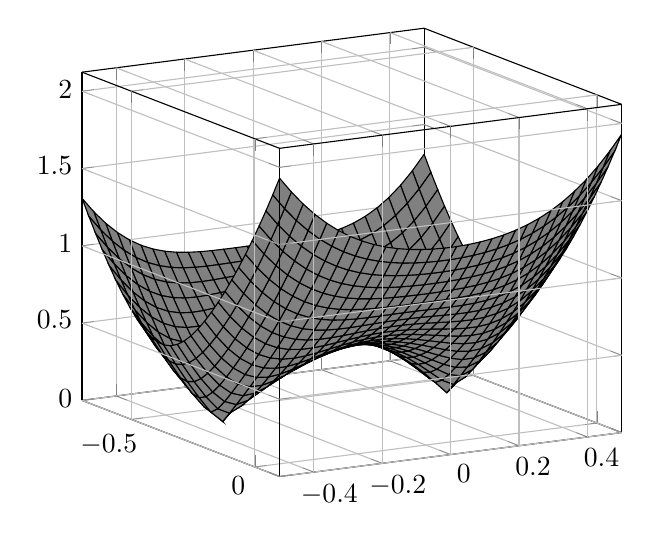
\begin{tikzpicture}
        \begin{axis}[view={60}{15},zmin=0,grid,
            3d box = complete*]
        \addplot3 [
            domain=-0.7:0.1,
            domain y = -0.5:0.5,
            samples = 30,
            samples y = 30,
            surf,
            fill=black!50,
            faceted color=black] {((-4*((x+2)^2-y^2)+13*(x+2)-11)^2+(13*y-8*(x+2)*y)^2)^(1/2)};
        \end{axis}
    \end{tikzpicture}
    \caption{Primera iteración}
    \label{first_poly}
\end{figure}
\begin{figure}
    \centering
    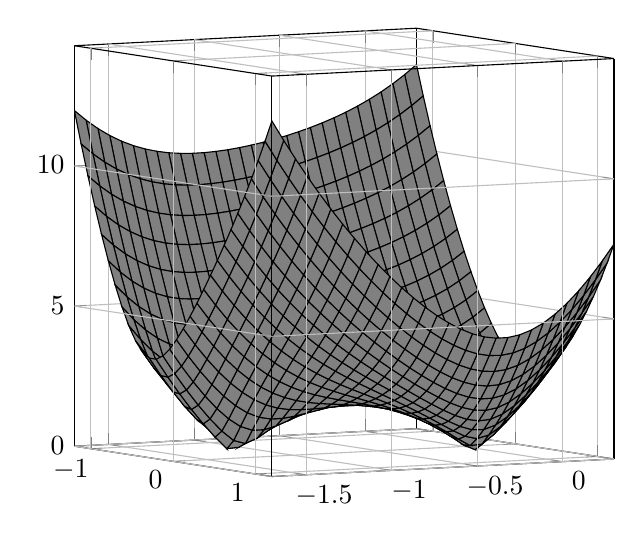
\begin{tikzpicture}
        \begin{axis}[view={60}{5},zmin=0,grid,
            3d box = complete*]
        \addplot3 [
            domain=-1.2:1.2,
            domain y = -1.7:0.3,
            samples = 30,
            samples y = 30,
            surf,
            fill=black!50,
            faceted color=black] {((0.330719*x^2-8.75*x*y-5.2915*x-0.330719*y^2+1.57092)^2+(-4.375*x^2-0.661438*x*y+2*x+4.375*y^2+5.2915*y+0.46875)^2)^(1/2)};
        \end{axis}
    \end{tikzpicture}
    \caption{Segunda iteración}
    \label{second_poly}
\end{figure}
\begin{figure}
    \centering
    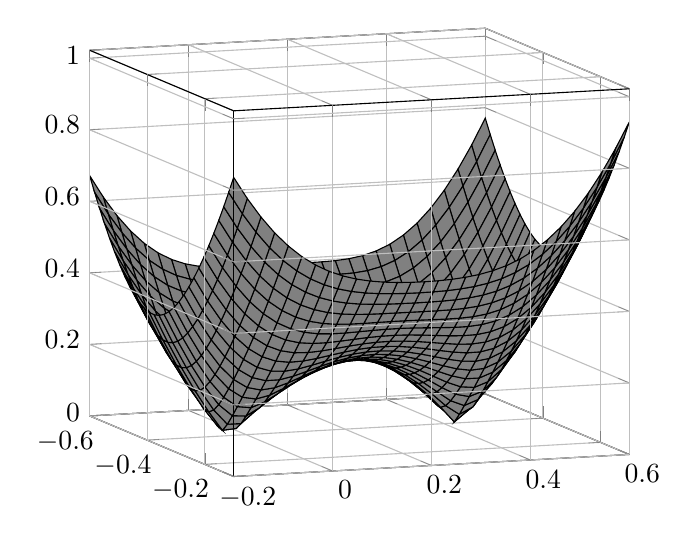
\begin{tikzpicture}
        \begin{axis}[view={70}{10},zmin=0,grid,
            3d box = complete*]
         
        \addplot3 [
            domain=-0.6:-0.1,
            domain y = -0.2:0.6,
            samples = 30,
            samples y = 30,
            surf,
            fill=black!50,
            faceted color=black] {((0.844055*x^2-7.59798*x*y+2.0208*x-0.844055*y^2-2.58721*y+0.665431)^2+(-3.79899*x^2-1.68811*x*y-2.58721*x+3.79899*y^2-2.0208*y-0.511867)^2)^(1/2)};
        \end{axis}
    \end{tikzpicture}
    \caption{Tercera iteración}
    \label{third_poly}
\end{figure}
\begin{table}[h!]
    \centering
    \caption{iteraciones del método.}
    \label{iterations_table}
    \begin{tabular}{c|c|c}
        \textbf{Iteración} & \textbf{Raíz 1} & \textbf{Raíz 2}\\
        \hline
        1 & $+1.625000+0.330718i$ & $+1.625000-0.330718i$\\
        2 & $+0.219445-1.020150i$ & $+0.326009-0.148102i$\\
        3 & $-0.381386-0.049646i$ & $-0.380227+0.412363i$\\
    \end{tabular}
\end{table}
El cuadro \ref{iterations_table} muestra las sucesivas aproximaciones de las raíces de los polinomios interpolantes
hacia la tercera raíz de la función original $(-0.419643+0.606290i)$, siendo que con únicamente tres iteraciones la
magnitud de la distancia de la raíz más cercana del tercer polinomio interpolante y la raíz de la función original es
de tan solo $0.197892$. Dos iteraciones más garantizan que $|f(x_n)<\epsilon|$ si se asume $\epsilon=10^{-6}$.